\chapter{Analyse des besoins et conception}

\section{Introduction}

Après avoir présenté le cadre général du projet, ce chapitre détaille l’analyse des besoins et la conception de la plateforme Virtual FabLab. L’objectif est de formaliser les fonctionnalités attendues, les contraintes de qualité, les acteurs du système, puis de proposer une architecture technique cohérente avec l’implémentation réalisée.

La conception retenue s’appuie sur une application web composée d’un frontend interactif, d’un backend applicatif, d’une base de données, d’un flux MQTT simulé et d’un module d’analyse de données.

\section{Étude des besoins}

L’étude des besoins vise à identifier les services que la plateforme doit fournir aux utilisateurs. Le système doit répondre à deux catégories principales d’utilisateurs : les étudiants et les administrateurs.

L’étudiant doit pouvoir accéder au FabLab virtuel, consulter les machines disponibles, réserver un créneau et tester un fichier de fabrication dans une simulation 3D. L’administrateur doit disposer d’un espace de pilotage lui permettant de gérer les machines, les utilisateurs, les réservations et les indicateurs de supervision.

Le système doit également être capable de recevoir des données simulées issues des machines, de les stocker et de les exploiter pour la détection d’anomalies et l’aide à la maintenance. Les données utilisées dans cette version sont simulées afin de valider l’architecture, les flux MQTT, le monitoring et le module d’analyse. La plateforme reste conçue pour être connectée ultérieurement à des capteurs réels.

\section{Besoins fonctionnels}

\subsection{Besoins de l’étudiant}

Les fonctionnalités attendues pour l’étudiant sont les suivantes :

\begin{itemize}
    \item créer un compte utilisateur ;
    \item s’authentifier et accéder à un espace personnel ;
    \item consulter les machines disponibles dans le FabLab ;
    \item visualiser le laboratoire virtuel en 3D ;
    \item sélectionner une machine et consulter ses informations ;
    \item effectuer une demande de réservation sur un créneau disponible ;
    \item consulter l’historique de ses réservations ;
    \item importer un fichier G-code ou NC compatible ;
    \item lancer, mettre en pause et réinitialiser une simulation ;
    \item modifier les informations de son profil.
\end{itemize}

\subsection{Besoins de l’administrateur}

Les fonctionnalités attendues pour l’administrateur sont les suivantes :

\begin{itemize}
    \item consulter un tableau de bord global ;
    \item gérer les utilisateurs et leurs rôles ;
    \item activer ou désactiver un compte utilisateur ;
    \item créer, modifier ou supprimer des machines ;
    \item modifier l’état et le placement 3D des machines ;
    \item consulter les demandes de réservation ;
    \item approuver, refuser ou supprimer une réservation ;
    \item superviser les données de télémétrie reçues ;
    \item suivre l’état MQTT du système ;
    \item consulter les alertes d’anomalies ;
    \item consulter les scores de santé et les recommandations de maintenance ;
    \item interroger un Copilote IA de maintenance pour obtenir une synthèse structurée fondée sur les données disponibles.
\end{itemize}

\section{Besoins non fonctionnels}

Les besoins non fonctionnels définissent les qualités attendues de la solution :

\begin{itemize}
    \item \textbf{Sécurité} : les fonctionnalités sensibles doivent être protégées par authentification et contrôle de rôle.
    \item \textbf{Ergonomie} : l’interface doit être claire, lisible et adaptée à un usage pédagogique.
    \item \textbf{Maintenabilité} : le code doit être organisé en modules séparant les responsabilités.
    \item \textbf{Évolutivité} : la solution doit permettre l’ajout de nouveaux types de machines ou de nouveaux indicateurs.
    \item \textbf{Performance} : la scène 3D et la simulation doivent rester fluides dans un navigateur moderne.
    \item \textbf{Traçabilité} : les données de télémétrie doivent être conservées afin d’alimenter l’historique et les analyses.
    \item \textbf{Interopérabilité} : les échanges entre frontend et backend doivent être réalisés à travers des API structurées.
\end{itemize}

\section{Acteurs du système}

Le système met en interaction plusieurs acteurs :

\begin{itemize}
    \item \textbf{Étudiant} : utilisateur inscrit qui consulte les machines, réserve des créneaux et lance des simulations.
    \item \textbf{Administrateur} : utilisateur disposant de droits avancés pour gérer la plateforme et superviser les machines.
    \item \textbf{Broker MQTT} : composant intermédiaire chargé de transmettre les messages de télémétrie simulée.
    \item \textbf{Machine simulée} : source logique des données de fonctionnement publiées dans le système.
\end{itemize}

\section{Cas d’utilisation}

Le diagramme de cas d’utilisation permet de représenter les interactions principales entre les acteurs et la plateforme.

\begin{figure}[H]
\centering
\IfFileExists{images/diagrame_user.png}
{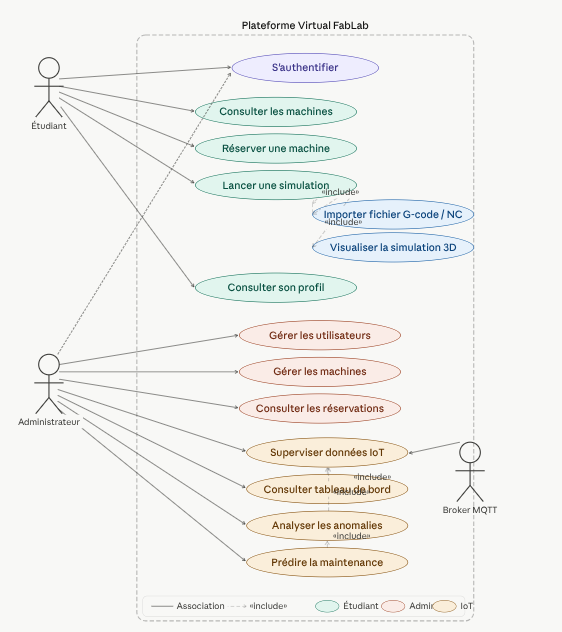
\includegraphics[width=0.95\textwidth]{images/diagrame_user.png}}
{\fbox{\parbox[c][5cm][c]{0.85\textwidth}{\centering Emplacement réservé pour le diagramme de cas d’utilisation\\\texttt{images/diagrame\_user.png}}}}
\caption{Diagramme de cas d’utilisation de la plateforme Virtual FabLab}
\label{fig:diagramme-cas-utilisation}
\end{figure}

Les cas d’utilisation principaux sont l’authentification, la consultation des machines, la réservation, la simulation, la gestion administrative, la supervision IoT et l’analyse des anomalies.

\section{Architecture générale}

L’architecture générale de la plateforme repose sur une séparation claire entre l’interface utilisateur, les services backend, la base de données, le flux MQTT et le module Data Science.

\begin{figure}[H]
\centering
\IfFileExists{images/architecture_generale.png}
{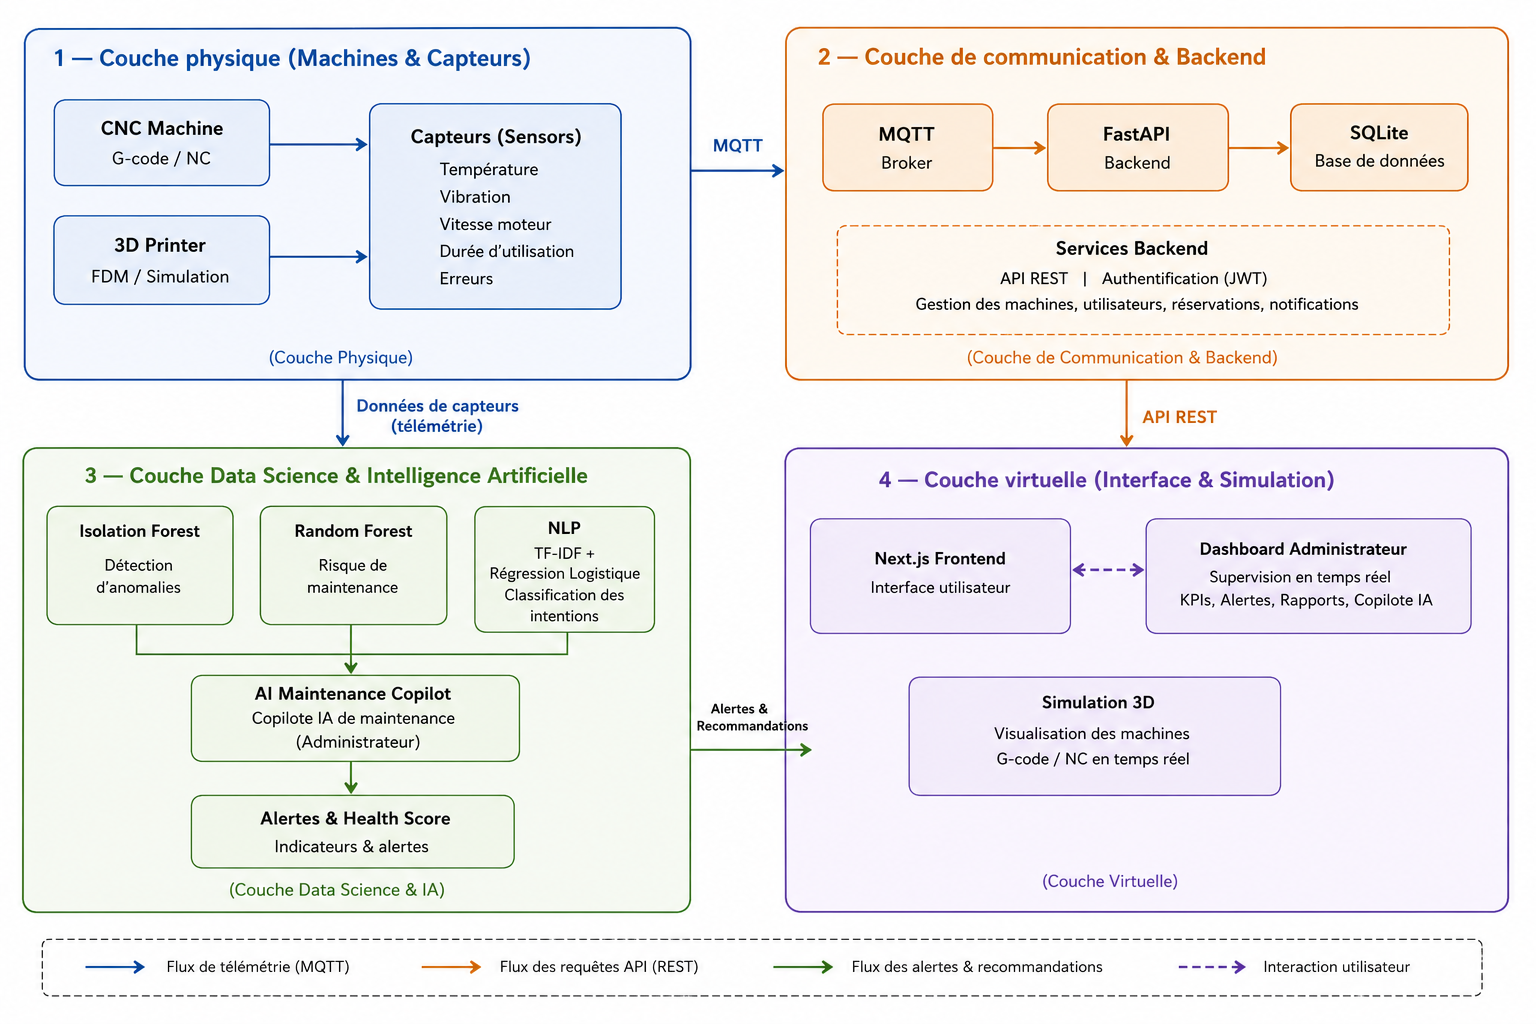
\includegraphics[width=0.95\textwidth]{images/architecture_generale.png}}
{\fbox{\parbox[c][5.5cm][c]{0.85\textwidth}{\centering Emplacement réservé pour le schéma d’architecture générale\\\texttt{images/architecture\_generale.png}}}}
\caption{Architecture générale de la plateforme Virtual FabLab}
\label{fig:architecture-generale}
\end{figure}

Le frontend communique avec le backend à travers des requêtes HTTP. Le backend expose les API, gère la base de données SQLite et lance un abonné MQTT au démarrage de l’application. Les messages reçus sont transformés en mesures de télémétrie puis exploités par les services de monitoring et de prédiction.

\section{Description des modules}

La plateforme est structurée autour des modules suivants :

\begin{itemize}
    \item \textbf{Module d’authentification} : inscription, connexion, profil, changement de mot de passe et génération de jetons JWT.
    \item \textbf{Module utilisateurs} : liste, recherche, changement de rôle et activation ou désactivation des comptes.
    \item \textbf{Module machines} : gestion des types de machines, des instances, de leurs états et de leurs coordonnées dans le laboratoire 3D.
    \item \textbf{Module réservations} : création des demandes, calcul des créneaux disponibles, annulation et validation par l’administrateur.
    \item \textbf{Module FabLab 3D} : visualisation interactive de la salle et des machines avec sélection et consultation de leur état.
    \item \textbf{Module simulation} : importation et interprétation des fichiers G-code ou NC pour l’imprimante 3D et la CNC.
    \item \textbf{Module MQTT} : réception des données simulées publiées sur les topics machines.
    \item \textbf{Module Data Science et IA} : détection d’anomalies avec Isolation Forest, estimation du risque de maintenance avec Random Forest Classifier, calcul du score de santé, classification supervisée des intentions administrateur et Copilote IA d’aide à la décision.
    \item \textbf{Module notifications} : notification des étudiants après validation ou refus d’une réservation.
\end{itemize}

\section{Diagramme de classes}

Le diagramme de classes représente les entités principales utilisées dans la base de données et leurs relations : utilisateur, machine, type de machine, réservation, mesure capteur et notification.

\begin{figure}[H]
\centering
\IfFileExists{images/class.png}
{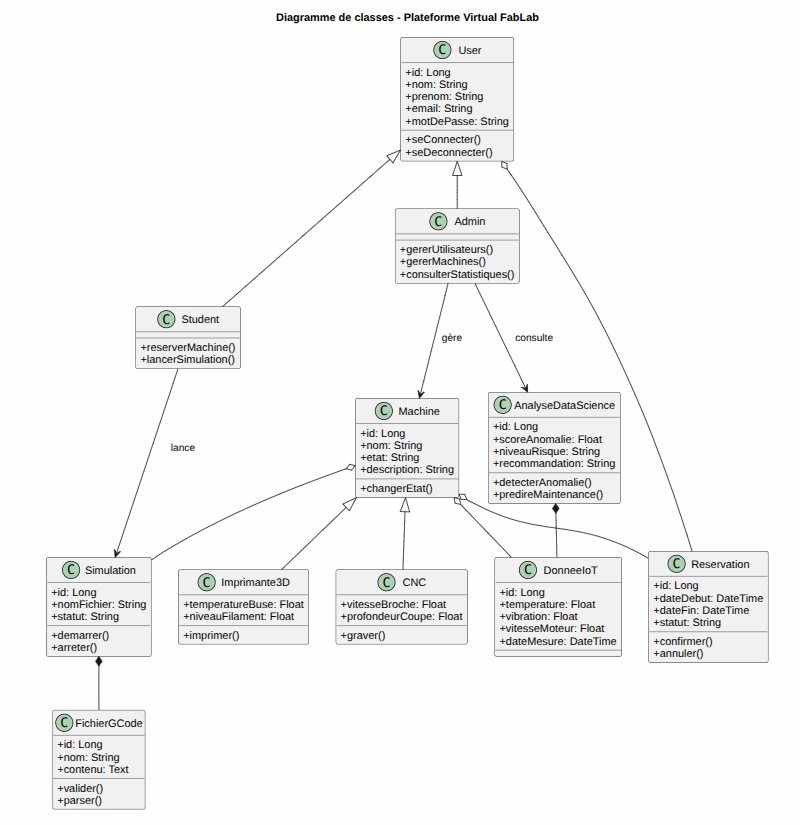
\includegraphics[width=0.95\textwidth]{images/class.png}}
{\fbox{\parbox[c][5cm][c]{0.85\textwidth}{\centering Emplacement réservé pour le diagramme de classes\\\texttt{images/class.png}}}}
\caption{Diagramme de classes de la plateforme Virtual FabLab}
\label{fig:diagramme-classes}
\end{figure}

La conception des données distingue les types de machines des instances de machines. Cette séparation permet d’associer un modèle 3D, un schéma de capteurs et des informations techniques à un type, tout en laissant chaque instance posséder son propre nom, état et emplacement.

\section{Conception du système}

\subsection{Conception de l’authentification}

Le système d’authentification repose sur des jetons JWT. Après connexion, le backend renvoie un jeton d’accès utilisé par le frontend pour appeler les routes protégées. Le rôle de l’utilisateur permet de distinguer les droits d’un étudiant et ceux d’un administrateur.

\subsection{Conception de la gestion des machines}

Chaque machine possède un type, un nom unique, un état, des notes et des paramètres de placement dans la scène 3D. Les machines peuvent être consultées par les utilisateurs, tandis que leur création, modification ou suppression est réservée à l’administrateur.

\subsection{Conception de la réservation}

Le système de réservation repose sur des créneaux d’une heure entre 8h00 et 20h00. Une demande est créée avec l’état \texttt{pending}. L’administrateur peut ensuite l’approuver ou la refuser. Les conflits sont évités en vérifiant les réservations actives pour la même machine et le même intervalle.

\subsection{Conception de la télémétrie}

Dans l’implémentation actuelle, la télémétrie simulée est reçue sous forme de messages JSON publiés via MQTT. Le backend associe chaque message à une machine existante, enregistre les mesures et expose l’historique à travers les routes de monitoring.

\subsection{Conception de l’analyse intelligente}

Le module Data Science et IA combine des modèles entraînés avec scikit-learn et une logique par règles. La détection d’anomalies s’appuie sur un modèle \textit{Isolation Forest}, tandis que l’estimation du risque de maintenance repose sur un \textit{Random Forest Classifier}. Une logique complémentaire par règles est utilisée pour consolider le score de santé, le niveau de risque et les recommandations de maintenance, notamment lorsque les modèles ne sont pas disponibles ou lorsqu’une lecture doit être interprétée de manière explicable.

Les variables analysées sont la température, la vibration, la durée d’utilisation exprimée sous forme \texttt{usage\_duration} puis convertie en \texttt{usage\_hours}, la vitesse du moteur \texttt{motor\_speed} et l’historique des erreurs signalées. Les sorties produites par le module sont le statut d’anomalie, la probabilité indicative de risque, le score de santé, le niveau de risque et une recommandation de maintenance.

Le même module intègre également une classification supervisée des intentions administrateur, fondée sur TF-IDF et Logistic Regression, afin d’alimenter un Copilote IA de maintenance. Ce copilote ne correspond pas à un LLM ni à une IA générative ; il fournit des réponses déterministes construites à partir des données de la plateforme, des résultats analytiques et de l’intention reconnue.

\section{Technologies utilisées}

\newcommand{\techitem}[3]{%
  \subsection{#1}
  \noindent
  \begin{minipage}[c]{0.22\textwidth}
    \centering
    \IfFileExists{#2}
    {\includegraphics[width=0.85\linewidth,height=1.8cm,keepaspectratio]{#2}}
    {\fbox{\parbox[c][1.8cm][c]{0.85\linewidth}{\centering\scriptsize #1}}}
  \end{minipage}
  \hfill
  \begin{minipage}[c]{0.72\textwidth}
    #3
  \end{minipage}
  \par\vspace{0.4cm}
}

\techitem{Next.js}{images/nextjs.png}{Next.js est un framework basé sur React permettant de développer des applications web modernes, modulaires et performantes. Dans ce projet, il constitue la base du frontend. Il organise les pages de l’application, les composants d’interface, les appels API et les vues interactives destinées aux étudiants et aux administrateurs.}

\techitem{FastAPI}{images/fastapi.jpg}{FastAPI est un framework Python destiné à la création d’API web rapides et structurées. Il est utilisé pour implémenter le backend de la plateforme : authentification, gestion des machines, réservations, monitoring, réception MQTT et services d’analyse.}

\techitem{Three.js}{images/threejs.png}{Three.js est une bibliothèque JavaScript permettant de créer des scènes 3D dans le navigateur. Elle est utilisée pour afficher le laboratoire virtuel, charger les modèles GLB des machines et animer les trajectoires issues des fichiers de fabrication.}

\techitem{Blender}{images/blender.png}{Blender est un logiciel de modélisation 3D open source. Il intervient dans la préparation et l’optimisation des modèles 3D utilisés dans la plateforme, notamment ceux de l’imprimante 3D et de la machine CNC.}

\techitem{MQTT}{images/mqtt.png}{MQTT est un protocole léger de communication publish/subscribe très utilisé dans les systèmes IoT. Dans ce projet, il permet de simuler l’envoi de mesures machines vers le backend à l’aide d’un simulateur MQTT. Les messages sont publiés sur des topics propres à chaque machine, selon le motif suivant :

\begin{center}
\small\texttt{fablab/machines/\{machine\_id\}/data}
\end{center}}

\techitem{Python}{images/python.png}{Python est utilisé côté backend pour développer les services applicatifs et les traitements de données. Il facilite également l’intégration des bibliothèques de Data Science et l’entraînement des modèles.}

\techitem{Tailwind CSS}{images/tailwind.png}{Tailwind CSS est un framework CSS utilitaire permettant de construire rapidement des interfaces cohérentes et responsives. Dans la plateforme, il est utilisé pour structurer les pages, les cartes, les tableaux, les formulaires et les tableaux de bord.}

\techitem{Scikit-learn}{images/scikit_learn.png}{Scikit-learn est une bibliothèque Python dédiée au Machine Learning. Elle est utilisée dans ce projet pour entraîner et exploiter un modèle de détection d’anomalies de type Isolation Forest et un Random Forest Classifier pour l’estimation du risque de maintenance.}

\techitem{Visual Studio Code}{images/vscode.png}{Visual Studio Code est l’environnement de développement utilisé pour organiser et modifier les différents modules du projet : frontend, backend, simulation, scripts Python et fichiers LaTeX du rapport.}

\newcommand{\iotitem}[3]{%
  \subsubsection{#1}
  \noindent
  \begin{minipage}[c]{0.22\textwidth}
    \centering
    \IfFileExists{#2}
    {\includegraphics[width=0.85\linewidth,height=1.8cm,keepaspectratio]{#2}}
    {\fbox{\parbox[c][1.8cm][c]{0.85\linewidth}{\centering\scriptsize #1}}}
  \end{minipage}
  \hfill
  \begin{minipage}[c]{0.72\textwidth}
    #3
  \end{minipage}
  \par\vspace{0.4cm}
}

\subsection{Technologies et équipements IoT}

Cette partie présente les composants matériels et les équipements de fabrication numérique liés à la dimension IoT du FabLab. Dans la version actuelle, ils servent de référence pour concevoir les mesures et les scénarios de supervision. La collecte effective n’est pas encore réalisée par des capteurs physiques : elle est simulée par MQTT afin de valider les flux, le stockage et l’analyse avant une intégration matérielle future.

\iotitem{ESP8266}{images/esp8266.jpg}{L’ESP8266 est un microcontrôleur doté d’une connectivité Wi-Fi intégrée, largement utilisé dans les applications de l’Internet des Objets. Dans un contexte FabLab, il peut servir d’interface entre les capteurs physiques et la plateforme de supervision. Il permet de collecter des mesures, de les traiter localement puis de les transmettre vers un serveur ou un broker MQTT. Son faible coût et sa facilité de programmation en font un choix adapté aux prototypes académiques et industriels légers.}

\iotitem{Capteur de température}{images/DHT.jpg}{Le capteur de température permet de mesurer l’échauffement d’un environnement, d’un composant électronique ou d’une machine en fonctionnement. Dans le cadre d’un FabLab intelligent, cette donnée est utile pour surveiller les conditions de travail et prévenir les situations anormales. Une température excessive peut indiquer une surcharge, un défaut de ventilation ou une dégradation progressive d’un équipement. Lors d’une connexion future à des capteurs réels, ces mesures pourront alimenter des tableaux de bord et des modèles de maintenance prédictive.}

\iotitem{Capteur de vibration}{images/capteur_vibration.jpg}{Le capteur de vibration mesure les oscillations mécaniques produites par une machine pendant son fonctionnement. Ces données sont essentielles pour les équipements de fabrication numérique, car des vibrations inhabituelles peuvent révéler un désalignement, une usure ou un défaut mécanique. Dans une approche de maintenance préventive, l’analyse de ces signaux aide à identifier les anomalies avant l’apparition d’une panne. Les données de vibration constituent ainsi un indicateur pertinent de l’état de santé des machines.}

\iotitem{Imprimante 3D}{images/imprimante_3d.png}{L’imprimante 3D est un équipement de fabrication additive permettant de produire des objets physiques à partir de modèles numériques. Elle fonctionne généralement par dépôt progressif de matière selon des trajectoires définies dans un fichier G-code. Dans un FabLab, elle constitue un outil pédagogique et technique essentiel pour le prototypage rapide. Son intégration à une plateforme IoT permet de suivre son état, sa température, sa progression et ses éventuelles anomalies de fonctionnement.}

\iotitem{Machine CNC}{images/cnc.jpg}{La machine CNC est un équipement de fabrication soustractive commandé numériquement. Elle exécute des opérations d’usinage à partir d’instructions précises, souvent décrites dans des fichiers NC ou G-code. Dans un FabLab, elle permet de travailler différents matériaux avec une grande précision. La supervision IoT d’une CNC peut porter sur son état, ses vibrations, sa durée d’utilisation et ses paramètres de fonctionnement afin d’améliorer la sécurité, la traçabilité et la maintenance.}

\section{Conclusion}

Ce chapitre a présenté l’analyse des besoins, les acteurs, les cas d’utilisation et la conception générale de la plateforme. Il a également décrit les technologies retenues et leur rôle dans le projet.

Le chapitre suivant sera consacré à la réalisation et à l’implémentation. Il détaillera l’organisation concrète du frontend et du backend, les modules développés, la simulation 3D, le flux MQTT et les interfaces de supervision.
